\chapter{抽 搐}

抽搐(convulsion)是部分或全身骨骼肌不自主、节律性的抽动,伴或不伴意识障碍,是临床上常见的症状。通常,按引起抽搐的病变部位分为脑源性、脊髓性、外周神经性和肌肉本身病变;按抽搐波及范围分为全身性和部分性,前者为全身骨骼肌的抽动,常伴意识丧失;后者局限于一侧肢体、一个肢体或仅面部肌肉的抽动,通常不伴有意识丧失;按抽搐形式可分为强直性(骨骼肌持续、强烈、非颤抖性收缩)、阵挛性(骨骼肌收缩和松弛交替出现)和肌阵挛性(骨骼肌突发、短暂、闪电样收缩)。伴发有肢体和肌肉疼痛的抽搐称为痛性抽搐。从疾病单元来说,抽搐包含有痫性发作和非痫性发作两大内容。

痫性发作(epileptic
seizure)是由于脑神经元过度兴奋或高度同步化活动产生的一过性症状,它的起始、中止和临床表现均有一定的特殊模式。而癫痫(Epilepsy)则是以脑部持续存在产生癫痫发作的易感性,由此而产生神经生理,认知功能,心理和社会障碍为特征的一种慢性脑部疾病。根据2005年国际抗癫痫联盟对癫痫最新定义,至少有一次癫痫发作才能诊断癫痫。

因此,抽搐、痫性发作和癫痫之间存在一定差异。应当清楚地说:抽搐不等于癫痫发作;癫痫发作可有抽搐,也可以不伴有抽搐;一次痫性发作不等于癫痫,但有癫痫者常有全身或局灶性抽搐。

\section{【抽搐的病理生理机制】}

抽搐既可以是遗传性代谢疾病的重要症状之一,也可由后天因素:如中枢神经系统疾病、周围神经系统疾病和中毒、代谢性疾病所引起。引起抽搐的病理生理机制复杂,因病变部位不同而有别。

\subsection{(一)脑源性抽搐}

脑源性抽搐由脑部神经元异常兴奋和同步放电所引起。许多机制如离子通道功能、神经递质水平、神经受体调节、能量代谢,以及调控这些机制的基因改变都可能引起皮质神经元的兴奋性增加,当脑的局部或全脑神经元以一种异常同步化的形式被激活时,就会引发痫性放电和出现临床抽搐发作。

神经系统先天或遗传因素可以作为痫性活动的病因和病理基础。如基因突变改变神经细胞膜离子通道的构型,导致离子的异常跨膜运动:目前发现与癫痫有关的基因多是通过调控钾、钙、钠、氯离子通道异常跨膜运动引起癫痫发作的。基因突变引起脑发育异常也可导致癫痫,其中以脑神经元异位征最常见。很多基因突变是通过代谢途径引起癫痫发作,尤其是线粒体突变对正常脑部的代谢影响更大:如伴破碎红纤维的肌阵挛、进行性肌阵挛性癫痫、Lafora病、Unverricht-Lundborg病等都是由于基因突变引起代谢功能障碍,从而导致癫痫。对离子通道基因突变的离体研究还发现,受体功能和结构异常是癫痫发生的一个重要原因。目前已知的癫痫基因中相当部分与受体有关,如常染色体显性夜间发作性额叶癫痫是一种新发现的遗传性部分性癫痫,基因克隆发现20号染色体长臂调控神经元烟碱型乙酰胆碱受体α4亚基基因有突变;之后在挪威家系中又发现15号染色体上有另一个突变点,呈现出遗传异质性。此外,目前对GABA能系统遗传学研究提示GABA能A受体基因异常是癫痫发生的重要机制。突触功能的异常,特别是化学突触功能异常是神经元兴奋性增加的主要原因。

后天获得的许多疾病,如脑血管疾病、外伤、药物中毒、代谢性疾病都可引起细胞水肿及神经元膜通透性改变,钠离子及其他离子异常内流,引起细胞外离子浓度和电阻增加,这些改变引发细胞及组织的兴奋性增加。脑发育畸形、脑内新生物引起的癫痫患者中都能见到胶质增生,这种异常的胶质细胞可通过多种途径点燃癫痫。代谢紊乱,如低氧、低糖影响神经细胞的能量代谢,改变了细胞膜内、外离子分布的正常梯度,降低了膜的稳定性,导致神经元兴奋性增加。

理论上讲,脑的任何部位受到刺激都可能引起脑神经元兴奋性改变导致癫痫发作,但某些部位脑神经元对癫痫的敏感性高、发作阈值低,更易成为癫痫病灶。目前发现对癫痫最敏感的是新皮质、旧皮质、脑干及嗅皮质。其中新皮质的癫痫发作可以干扰人体的感觉和运动功能,出现相应的临床表现。目前研究表明:脑干是产生癫痫的一个重要部位,直接刺激脑干可引起最大惊厥和次最大强直-阵挛性发作,网状核团的刺激可在前脑完全无放电的情况下引发全身性发作。这种脑干点燃的痫性活动能够自身维持,即使是单侧刺激也可引发双侧抽搐,证实脑干有维持和产生全身性惊厥所必需的神经环路。在四叠体上方阻断前脑与脑干的联系,仍不能阻止电或化学刺激脑干所引起的强直性发作,证实脑干是独立于前脑的一个易产生癫痫的部位。某些强直-阵挛性发作起至脑干,网状结构全部活动产生强直性惊厥,部分活动则产生阵挛,破坏可抑制癫痫发作。

\subsection{(二)非脑源性抽搐}

非脑源性抽搐系指由于脊髓网状结构兴奋引起下运动神经元的γ纤维兴奋而致肢体强直收缩,如马钱子、士的宁中毒引起的肢体抽搐。周围神经病的面神经炎后遗症可出现面肌抽搐。钙离子代谢障碍和甲状腺手术后的手足搐搦等,均是肌细胞膜兴奋性增高所引起的肢体抽搐。

\section{【病因】}

引起抽搐的原因很多,大致上可分为由脑部疾病和非脑部疾病所致的抽搐两大类:

\subsection{(一)脑部疾病(脑源性抽搐)}

多表现为癫痫的形式。

\subsubsection{1.特发性或隐源性癫痫}

是引起肢体抽搐较为常见的病因,脑电图提示为普遍性、双侧对称同步性的异常放电,发作间期可表现正常,无神经系统体征和神经影像学征象。常见类型有早期肌阵挛脑病、肌阵挛站立不能性癫痫、青少年肌阵挛型癫痫、进行性肌阵挛型癫痫、热性惊厥。

\subsubsection{2.症状性癫痫}

颅内器质性病变常可引发癫痫发作,表现为局部和全身肢体的抽搐,脑电图提示为局灶性或全面性异常放电,多伴有神经系统阳性体征和神经影像学的异常。常见病因有颅内肿瘤、脑血管病、脑感染性疾病、外伤性、先天发育异常和遗传代谢性疾病。

\paragraph{(1)颅内肿瘤:}

大脑半球额叶、中央皮质区的肿瘤均可引起抽搐。按肿瘤分化来源不同分为原发性肿瘤(少突胶质细胞瘤、星形胶质细胞瘤Ⅰ~Ⅱ级、脑膜瘤、颅咽管瘤、髓母细胞瘤等)和继发性肿瘤即脑转移瘤。

\paragraph{(2)脑血管病:}

脑动静脉血管畸形、脑动脉瘤、脑栓塞(心源性栓子、外伤性气栓、脂肪栓)、脑动脉血栓形成、脑静脉窦血栓形成、脑出血、蛛网膜下腔出血、无脉病、高血压脑病。

\paragraph{(3)脑感染性疾病:}

病毒感染(单纯疱疹病毒性脑炎、日本乙型脑炎病毒性脑炎、病毒性脑膜脑炎等)、细菌感染(化脓性脑膜炎、脑脓肿、结核性脑膜炎等)、真菌感染(隐球菌性脑膜炎、毛霉病等)、脑寄生虫病(脑血吸虫病、脑囊虫病、脑肺吸虫病、脑包虫病、弓形虫病、脑型疟疾)、肉芽肿(结核性肉芽肿、真菌性肉芽肿、寄生虫性肉芽肿、血管炎性肉芽肿、结节肿)、神经梅毒。

\paragraph{(4)外伤性:}

颅内血肿后、脑挫裂伤、脑穿通伤及火器伤、产伤。

\paragraph{(5)先天性发育异常:}

小头畸形、狭颅症、脑发育不全、先天性脑穿通畸形、先天性脑积水、先天性胼胝体发育不全。

\paragraph{(6)遗传代谢性疾病:}

①脂质累积病:家族性黑蒙性痴呆、脑白质营养不良症、肾上腺皮质营养不良症糖;②原累积病;③结节性硬化(tuberous
sclerosis);④氨基酸代谢障碍病:苯丙酮尿症;⑤脑面血管瘤病(Sturge-Weber
syndrome);⑥脆性X综合征等。

\subsection{(二)非脑部疾病}

\subsubsection{1.全身感染性疾病}

急性胃肠炎;中毒型菌痢;败血症;中耳炎;百日咳;狂犬病;破伤风等。

\subsubsection{2.全身代谢性疾病}

发热性疾病如热性惊厥;肺性脑病;肾性脑病;肝性脑病;低血糖症;水、电解质紊乱(严重脱水、低钠血症、低钙血症、低镁血症)急性间歇性血卟啉病;子痫;维生素B\textsubscript{6}
缺乏症等。

\subsubsection{3.全身中毒性疾病}

植物源性中毒(马钱子中毒、白果中毒、咖啡因中毒、乌头中毒等);动物源性中毒(毒虫叮咬、毒蛇咬伤等);化学物质性中毒(有机磷农药、苯、铅、汞、砷、等);药物性中毒(洋地黄、阿托品、丙氧酚、丙咪嗪等)等。

\subsubsection{4.自身免疫性疾病}

系统性红斑狼疮、脑血管炎等。

\subsubsection{5.缩窄性周围神经病}

面肌抽搐、痛性肌痉挛。

\subsubsection{6.其他}

撤药诱发(抗癫痫药和镇静催眠药)、酒精戒断综合征等。

\subsection{(三)功能性抽搐}

癔症性抽搐。

\section{【抽搐的临床类型】}

按照发作时累及的部位、形式和是否伴有意识障碍,临床上抽搐可分为下列几种类型:

\subsection{(一)全身强直-阵挛抽搐}

是临床最常见的一种形式。主要特征为突然意识丧失、跌倒、四肢抽搐,先表现为强直(全身骨骼肌呈持续性收缩),持续约10~20秒;随后肢端出现细微震颤而转入阵挛期,即全身不同肌群强直和松弛交替出现,由肢端延及全身。阵挛频率逐渐减慢,松弛期逐渐延长持续约0.5~1分钟。最后一次强直痉挛后抽搐停止。每次2~5分钟。这种形式的抽搐既可以是原发性癫痫大发作的典型临床表现,也可见于由脑炎、脑膜炎、中毒代谢性脑病继发的症状性癫痫以及热性惊厥等。

\subsection{(二)全身强直性抽搐}

是一种全身肌肉强烈而又持续地收缩,常使肢体固定在某种紧张的位置。常见的是头眼偏向一方或后仰、上肢内旋、下肢挺直、躯干强直造成角弓反张,多数意识丧失,偶亦有意识清醒。常伴有自主神经症状,如面色苍白、潮红、瞳孔散大等。这类抽搐见于急性脑缺氧、脑炎、士的宁中毒、破伤风等,亦见于癫痫患者。

\subsection{(三)全身阵挛性抽搐}

几乎均发生在低龄儿童,主要是新生儿和婴儿。发作最先表现为意识丧失,伴突发肌张力降低,或短暂的、全身肌阵挛抽动致患者跌倒,接着出现不规则(以一侧或某一肢体为主,幅度、频率变化多端)全身肢体肌肉节律性抽动,节律快慢可变化,但某些儿童(尤其是1~3岁的患儿)为全身对称、同步的阵挛抽搐,持续1至数分钟。发作时自主神经功能改变相对少见,仅在发作持续时间长的患儿有呼吸道分泌物增多。此类发作多见于儿童发热性疾病,如发热惊厥。

\subsection{(四)肌阵挛性抽搐}

肌阵挛性抽搐为突然发生、短暂、不自主的肌肉收缩。可以遍及全身,也可局限于面部、躯干及一个或数个肢体;可以是单次受累肌群的反跳,也可以是多次重复肌阵挛反跳;可以是节律性的,也可以是不规则的;可以是癫痫发作,也可以是非痫性的。肌阵挛性癫痫或癫痫肌阵挛发作,在发作期脑电图可见棘波、多棘波、棘-慢和多-棘-慢复合波,同步肌电图可见短期(时程<59毫秒)暴发肌电活动。按其病因学分为遗传性和后天获得性的,前者可见于良性原发性癫痫综合征、重型肌阵挛癫痫综合征和进行性肌阵挛癫痫,后者见于因缺氧、脑外伤、脑肿瘤、尿毒症和其他代谢性脑病、中枢神经系统变性疾病、卒中和病毒感染等引起的症状性癫痫。而非痫性肌阵挛见于脊髓疾病、小脑性协同失调性肌阵挛、皮质下节段性肌阵挛等;发作期脑电图无痫性放电,同步肌电图示爆发长时程肌电活动(50~300毫秒)。

\subsection{(五)局限性抽搐}

局部肌肉或局部肢体发生抽搐,抽搐时意识清醒。可见于癫痫的局限性运动性发作;也可见于非痫性运动障碍,如阵挛性面肌抽搐、手足搐搦症等。

\section{【诊断过程】}

凡有抽搐者均应通过以下诊断过程明确性质。

\subsection{(一)病史询问}

详细而又准确可靠的病史是诊断的主要依据,当患者不能诉述发作经过时,需向目睹者仔细了解发作的全过程。病史询问中应注意:①首次发生抽搐的年龄,发作频度,每次发作的持续时间以及家族中有无类似发作史者;②发作前有否先兆或前驱症状,发作时有否意识丧失,发作过程是否能够回忆;③抽搐时姿势如何,有否因抽搐而伤害身体,如咬破舌头、跌破头部等;④发作时有否伴随出汗、心慌、脸色苍白还是潮红等自主神经症状;⑤伴随疾病,如伴随高血压、糖尿病、内分泌疾病、心脏病等情况,以及用药情况。

\subsection{(二)体格检查}

详细的内科和神经系统体格检查。一般智能检查,以便了解患者的智能情况、生长发育情况。神经系统体格检查的重点是了解是否肢体不对称性、局灶性神经系统损伤的阳性体征,为抽搐的定位、病因做出参考性诊断意见。

\subsection{(三)必要的辅助检查}

长程视频录像脑电图是鉴别癫痫性抽搐和非痫性抽搐关键的辅助检查,结构影像如头颅CT、MRI对脑部疾病引起的抽搐有定位和定性作用,而功能影像如SPECT、PET、fMRI不但对有明显脑部结构损害引起的抽搐有定位和定性作用,更可贵的是对仅有功能损害的脑部病变仍有定位定性诊断作用。血、尿常规检查,肝功能检查,特别是尿素氮及肌酐。查血糖、血清钙、磷等,以了解是否有代谢病所致的抽搐。

\section{【鉴别诊断】}

抽搐发作的鉴别诊断首先肯定是否抽搐,即真性抽搐还是假性抽搐;其次需鉴别癫痫性抽搐还是非癫痫性抽搐,癫痫性抽搐的发作类型;最后鉴别各种抽搐的原因。

\subsection{(一)真性抽搐还是假性抽搐}

真性抽搐是由颅内疾病、周围神经和脊髓疾病所致的抽搐,假性抽搐为癔症性抽搐。通常经详细病史询问,结合体格检查和血液检查不能发现内科代谢病或其他器质性疾病,神经系统检查排除颅内疾病,脑电图正常,头颅CT、MRI又无异常发现,应考虑假性抽搐。痫性抽搐与昏厥及癔症的鉴别见表\ref{tab51-1}。

\begin{table}[htbp]
\centering
\caption{痫性抽搐与昏厥及癔症的鉴别}
\label{tab51-1}
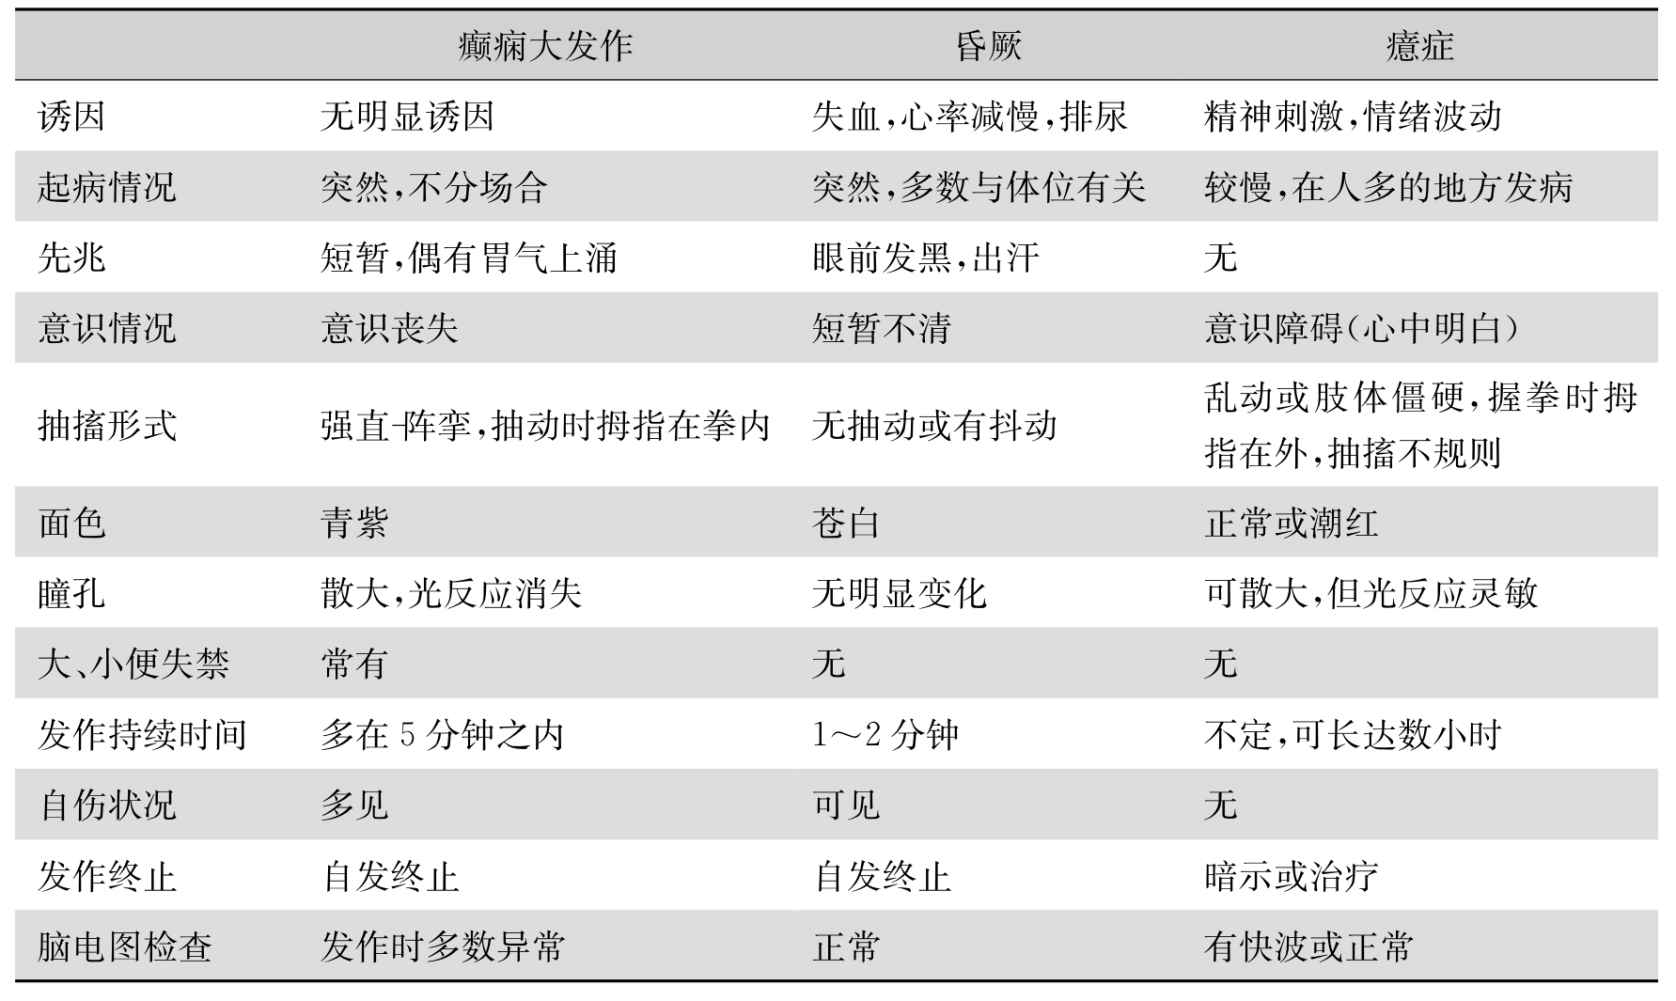
\includegraphics[width=5.9375in,height=3.54167in]{./images/Image00312.jpg}
\end{table}

\subsection{(二)何种类型的抽搐,明确是否属于痫性抽搐}

\subsubsection{1.痫性抽搐与热性惊厥的区别}

热性惊厥必须发生在婴儿或在5岁以内首次发生抽搐,6岁以后抽搐时虽然伴有发热,但仍不能诊断为热性惊厥,而必须诊断为惊厥。

\subsubsection{2.痫性抽搐与脑炎的区别}

痫性大发作后患者可遗留数分钟至数十分钟的意识障碍,表现为意识模糊、谵妄甚则昏迷,严重者可持续昏迷数小时至一天。多见于短期多次癫痫大发作或持续状态时,易被误诊为病毒性脑炎。凡一次抽搐发作后昏迷数小时后清醒,或连续多次抽搐发作,发作间歇期意识不清,并在抽搐终止后持续昏迷数天者,不能随便诊断为脑炎。仅脑脊液检查异常、弥漫性脑电图改变、头颅CT或MRI异常信号者,才能诊断为脑炎。

\subsection{(三)何种病因所致的抽搐}

血糖降低者为低血糖抽搐,要考虑胰岛细胞瘤的可能。手足搐搦症者常由血钙降低所致,应该考虑甲状腺功能低下或Fahr病性低钙性抽搐。肾功能异常、尿毒症者为代谢性抽搐。妊娠晚期伴高血压和尿蛋白水平异常者考虑子痫。局灶性抽搐常有定位意义,常能根据抽搐部位作出颅内相应部位的定位诊断,经检查确定疾病性质。凡痫性抽搐者,一般认为,新生儿、婴儿期发生的抽搐常与先天发育或产伤有关;学龄前开始至20岁之前首次发生抽搐发作者以原发性多见;10~50岁首次发生抽搐者以中枢神经系统感染(病毒性脑炎、寄生虫)、外伤、肿瘤等因素为多见;50岁以上者则应首先考虑血管性病变的可能。因此,必须注意抽搐在不同年龄组中有不同的病因。

\section{【各类抽搐的临床特征】}

\subsection{(一)特发性或隐源性癫痫引发抽搐}

\subsubsection{1.良性家族性新生儿惊厥}

良性家族性新生儿惊厥(benign familial neonatal
convulsion,BFNC)是新生儿期发病的癫痫综合征,由Rett等首次报道。本病存在着遗传异质性,按其表型和基因型不同分为良性家族性新生儿惊厥I型(BFNC1)和良性家族性新生儿惊厥Ⅱ型(BFNC2)。

\paragraph{(1)良性家族性新生儿惊厥I型(BFNC1):}

BFNC1为常染色体显性遗传病,由20q13.3上电压门控性钾通道基因KCNQ2基因突变引起。首次发作始于出生后第三天,6周内发作消失,发育过程正常。临床表现:开始为广泛性强直,继而出现自主神经症状(如呼吸暂停、心率改变等)、双侧或两侧游走的阵挛性抽搐及吸吮咀嚼等自动症。每次发作持续1~3分钟,第一周常有频繁发作、但少有持续状态,以后少量单次发作。在良性家族性新生儿惊厥/颤搐综合征,患儿相继出现良性家族性新生儿惊厥和肌肉抽搐。肌肉抽搐以肌纤维群自发地不自主收缩为特点,可见皮肤表面的蛆形运动,伴或不伴相应肌肉的僵硬和放松延迟,累及躯干、上肢、下肢肌肉,但不累及面部肌肉,发生于8~10岁之间。

\paragraph{(2)良性家族性新生儿惊厥Ⅱ型(BFNC2):}

BFNC2亦为常染色体显性遗传,由8q24上电压门控性钾通道基因KCNQ3突变所致。其表型与Ⅰ型相似,在起病后6~24个月内发作缓解。

\subsubsection{2.良性家族性婴儿惊厥}

良性家族性婴儿惊厥(benign infantile familial
convulsion,BIFC)是婴儿期发病的良性特发性癫痫综合征,由Vigevano等1990年首次报道。本病起病年龄为3~24月龄、高峰在4~8月龄。患儿围生期无异常,病前精神运动发育正常。起病初期多为成簇发作(持续1~3天),最多一天8~10次,间隔数十分钟至数小时不等;也有少数初期为孤立性发作,数天后成簇发作。发作时最常见的症状为活动明显减少或停止、两眼凝视,意识似有障碍;也可见头、眼向一侧偏转(方向每次发作不定),四肢肌张力增高或降低,面、唇青紫,口咽部自动症。惊厥症状可见一侧或双侧肢体阵挛性抽动,两侧可同步或先后出现,每次发作2~5分钟。发作后有短期的疲乏、嗜睡。起病1个月内可有孤立性发作或偶尔成簇发作,以后很少再复发。未经治疗的患儿1岁内可有少量散在的无热惊厥或热性惊厥。

神经系统检查正常、神经影像学检查无异常发现。发作间期脑电图正常,但成簇发作间期可见顶、枕区慢活动或棘波发放。发作时脑电图显示放电起自顶、枕区,从低波幅棘波节律开始,波幅逐渐增高,频率逐渐减慢并扩散到一侧半球乃至双侧半球。同一患儿各次发作的起源侧不定。发作后可有短暂抑制波或弥漫性慢活动。

所有患儿其发作均会停止,故预后良好,在有限的随访中未见精神运动衰退的报告。本病呈AD遗传,全基因和单倍型连锁分析提示存在遗传异质性。目前按基因型不同分为四型。BFIC
1基因位19q,BFIC2基因位16p12-p11D16S690和D16S685间的2.7-Mb区间。BFIC3起病年龄出生后3天至7月龄,有作者将这型定为良性家族性新生儿-婴儿惊厥(benign
neonatal-infantile familial
convulsion,BNIFC),其基因位2q24,现证实此型为SCN2A基因突变所致,目前已发现6种点突变,结果导致钠通道失活比率降低,离子跨膜运动增加从而兴奋性增高。Li等(2008)对一个4代8例BFIC中国大家系的全基因组和单倍型连锁分析发现该型不同前面三型,其基因座位在1p36.12-p35.1D1S2864和D1S2830之间12.4-cM区间,提示为BFIC4。

\subsubsection{3.早期肌阵挛脑病(early myoclonic encephalopathy)}

又称为早期肌阵挛癫痫性脑病。1978年由Aicardi和Goutiers首次报道。在1989年国际抗癫痫联盟提出的癫痫及癫痫综合征分类中,将本病列在全身发作的癫痫综合征一类。患儿生后3个月以内(多在1个月内)起病。有家族聚集性,提示可能为先天性代谢异常。病前未见脑发育异常。男女发病率大致相同。

本病有4种发作类型:①不固定或部分肌阵挛;②大范围肌阵挛;③单纯部分发作;④强直型婴儿痉挛。肌阵挛可表现为肢体或面部肌肉抽动。有时表现为眼睑或手指快速微小的抽动。肌阵挛发作频繁,有时呈持续状态。少数病例发作次数很少。强直型婴儿痉挛发作常在病程较晚期出现,大约在生后3~4个月出现,多在睡眠时发生,有时可连续反复发作。脑电图的正常背景波消失,代之以“爆发抑制(suppression
burst)”,爆发波是由无规律的高波幅慢波混有尖波、棘波所组成,持续1~5秒,随后为持续3~10秒的低波幅缺乏电活动的平坦波形。

\subsubsection{4.肌阵挛站立不能性癫痫(myoclonic-astatic epilepsy)}

又称为肌阵挛失张力性癫痫或Doose
syndrome。为小儿时期原发性全身型癫痫的一种,主要表现为肌阵挛及站立不能发作,常有遗传因素。发病年龄为7个月~6岁,94\%的患儿在5岁以内发病,以3~4岁发病最多,个别患儿在1岁以内发病。男女比例为2∶1。病前智力、运动功能发育正常。发病形式多样,常见轴性肌阵挛发作,以头、躯干为主,表现为突然、快速地用力点头、向前弯腰,同时两臂上举。有时肌阵挛发作很轻微,仅表现为眼睑和面部肌肉抽动或眼球快速运动。有时发作只表现为肌阵挛,但有时在肌阵挛后出现失张力发作,由于肌张力突然丧失而出现屈膝、跌倒、不能站立。有时可以见到强直-阵挛发作。

本综合征常可见到非惊厥性持续状态,表现为不同程度的意识混沌,表情呆滞或中等程度的感觉迟钝,有时呈木僵状态。持续状态还可表现为一连串的点头动作,及反复发作的肌张力丧失、跌倒。

\subsubsection{5.特发性全面性癫痫}

特发性全面性癫痫(idiopathic generalized
epilepsy,IGE)以反复全面强直-阵挛性发作为特征,无脑损害和(或)代谢异常。EEG表现为广泛的双侧同步对称性放电。包含IGE的各种综合征有:良性新生儿家族性惊厥、儿童失神癫痫(CAE)、青少年失神癫痫(JAE)、青少年肌阵挛性癫痫(JME)和觉醒期大发作癫痫(commission
on classification and terminology of the international league against
epilepsy,1989)。

按遗传学分型,IGE有若干亚型,不同的亚型与不同的基因有关。IGE的易感位点已经鉴定出来,如EIG1(8q24)、EIG2(14q23)、EIG3(9q32-q33)、EIG4(10q25-q26)、EIG5
(10p11.22)。EIG6与CACNA1H基因变异有关,EIG7与15q13.3的一处微缺失有关。有证据表明,苹果酶-2(malic
enzyme-2,ME2)可能是青春期特发性全面性癫痫发病的易感基础。已经检测到伴抑制爆发的新生儿肌阵挛癫痫存在线粒体谷氨酸盐转运体缺陷,基因基础是SLC25A22基因突变。

\subsubsection{6.青少年肌阵挛性癫痫}

青少年肌阵挛癫痫(juvenile myoclonic
epilepsy,JME),又称为前冲性癫痫小发作(impulsive petit
mal)、急跳性癫痫(jerk
epilepsy)、间歇性散发性肌阵挛性癫痫(intermittent sporadic myoclonic
epilepsy)或Janz综合征。

这种综合征较常见,约占所有癫痫的5.4\%~10.2\%,占特发性全面性癫痫的26\%。本病起病多为8~20岁的青少年,有明显的遗传倾向,男女性别无差异。临床表现为双臂的单次或反复的不规则、无节律的肌阵挛性急跳,有些患者可因此突然跌倒,无或仅有短暂的意识障碍。通常在早晨觉醒时发作,可被缺睡所诱发。患者为光敏性。大多数患者伴全身强直-阵挛性发作,这种全身强直-阵挛性发作可在肌阵挛后发生,或在其前出现,少数有失神发作,患者无明显智能缺陷。最常见的脑电图异常为双侧对称的4~6Hz多棘-慢复合波,15~30Hz的多棘波或2~3Hz棘-慢复合波。棘波和肌阵挛发作之间无密切的时相联系。而且EEG异常常见于患者的发作间期,多数节律性闪光刺激可诱发棘波、多棘波或棘-慢复合波甚至肌阵挛急跳。

JME是一种遗传异质性疾病,JME患者的家族中,JME和其他几种全身发作类型的发病率都高于普通人群。在无临床症状的家族成员中,异常脑电图(弥漫性棘-慢复合波或尖-慢复合波)的出现率也增高。连锁分析发现相同的临床表型可以由不同的基因突变引起,因此按照不同的连锁位点把JME分成4型:JME-1由6p12-p11的EFHC1基因突变所致,JME-2基因座位在15q14,JME-3基因座位在6p21,JME-4基因座位在5q12-14。另外,有报道4个基因突变与JME有关,包括5q34-q35的GABRA1基因、2q22-q23的CACNB4基因、3q26的CLCN2基因,1p36.3的GABRD基因。

本综合征对药物治疗反应良好。丙戊酸钠可以控制大多数JME患者的发作。

\subsubsection{7.良性成人家族性肌阵挛性癫痫}

良性成人家族性肌阵挛性癫痫(benign adult familial myoclonic
epilepsy,BAFME)又称伴癫痫症的家族性皮质肌阵挛震颤(familial cortical
myoclonic tremor with
epilepsy,FCMTE)。本病是一组罕见的癫痫综合征,多数家系来自日本的报道,所有资料显示其为常染色体显性遗传病,发病年龄在18~50岁,连锁分析显示存在遗传异质性。目前依据其基因座位的不同分为BAFME1和BAFME2

Ikeda等(1990)报道了2例日本患者。临床表现以发作性非进展性姿势性和动作性手指震颤为特点,有家族史。EMG显示与特发性震颤相似的9Hz节律波;SEP可见伴有增强的长环C-反射的巨大的体感诱发电位;EEG结果通过急跳锁定平均法确定运动前皮质的棘波发放,提示为皮质起源。本病用肾上腺素能β阻断剂治疗无效,但抗惊厥药如氯硝西泮、丙戊酸钠和扑米酮有效。Ikeda等得出结论:不自主运动或“皮质震颤”是皮质反射性肌阵挛的一种形式。Kuwano等(1996)描述了5个明显的常染色体显性遗传的BAFME日本家系。受累患者有肌阵挛、或癫痫和异常EEG表现,尤其EEG的光敏性。通过多个候选基因的连锁分析排除了已知合并肌阵挛的遗传代谢病。以后Terada等(1997)和Okino(1997)分别报道了3个家系9例患者确立了BAFME临床表型和电生理特征及良好的预后。但是,Elia等(1998)描述了一个常染色体显性遗传模式的皮质震颤、癫痫、精神发育迟滞的欧洲家族,4名存活的患者均具有BAFME电生理特征。3例有GTCS患者可用苯巴比妥和(或)地西泮得到良好控制。下一代的2名年龄最小的患者有更为严重的表型、出现症状更早(5岁)和中度精神发育迟滞。

\subsubsection{8.全面性癫痫伴发作性运动障碍}

全面性癫痫伴发作性运动障碍(generalized epilepsy and paroxysmal
dyskinesia,GEPD)为癫痫和发作性运动障碍共存于同一个体或同一家族。发作间期EEG示广泛的棘-慢复合波。家系分析提示为常染色体显性遗传。全基因组扫描显示该综合征由10q22的KCNMA1基因突变引起。由于离子通道在癫痫和发作性运动障碍如发作性共济失调中的重要性,推测编码离子通道的基因突变可能造成GEPD,并通过连锁分析确定了在8.4cM区域内编码离子通道的2个基因:VDAC2和KCNMA1。目前的研究并没有发现VDAC2的突变,但发现GEPD先证者的家族中KCNMA1基因10号外显子中一个杂合子发生了A向G的转化。

\subsubsection{9.进行性肌阵挛性癫痫}

该病为遗传异质性疾病,按其临床表现、遗传方式和致病基因的不同分为Unverricht-Lundborg病和Lafora型肌阵挛癫痫。

\paragraph{(1)Unverricht-Lundborg病:}

翁弗里希特-伦德伯格病(Unverricht-Lundborg
disease,ULD)又称为进行性肌阵挛性癫痫I型(epilepsy progressive
myoclonic
1,EPM1)或波罗的海肌阵挛型癫痫,为常染色体隐性遗传病。本病6到13岁发病,以惊厥为其临床特征。1~5年后出现肌阵挛。颤搐主要见于四肢近端肌肉,双侧尽管不同步但呈对称性。开始轻微,病程后期变得严重,甚至发作时患者被抛在地板上。有精神衰退,最终发展为痴呆。小脑性共济失调的体征在病程后期(常为10~20年)。总体而言,与Lafora病相比:ULD患者病情相对稳定、发作稀少、没有或有轻微精神损害,而Lafora病患者反复发作且精神状态恶化;ULD患者多表现为随意运动激发的动作性肌阵挛,而Lafora病患者是自发性肌阵挛。

Mascalchi等(2002)对基因检查确诊的10例ULD患者行MRI和MRS检查发现其脑桥基底部、小脑半球体积缩小,大脑也有轻度萎缩。后者有别于橄榄体脑桥小脑萎缩。这一发现证实ULD存在脑干和小脑通过丘脑皮质环路对大脑皮层抑制减少。

本病为常染色体隐性遗传病,基因座位在21q22.3。Pennacchio等(1996)研究证实ULD(或EPM1)的发生是由于抑半胱氨酸蛋白酶蛋白B基因(CSTB)突变所致。CSTB是一种半胱氨酸蛋白酶抑制剂,正常个体可以广泛表达,而ULD患者淋巴样干细胞中的表达明显减少。目前在ULD患者中已发现6种CSTB基因突变导致蛋白截断和或功能改变。

\paragraph{(2)Lafora型肌阵挛癫痫(myoclonic epilepsy of Lafora):}

本病由Lafora和Glueck(1911)首次描述,Ortiz-Hidalgo(1986)用显微镜观察到的神经细胞内的小体而命名。Lafora型肌阵挛癫痫属常染色体隐性遗传病。通常在15岁左右起病,最初表现为癫痫大发作和(或)肌阵挛发作,以后逐渐发生快速、严重的精神衰退,常伴有精神症状。本型预后差,发病后存活不超过10年。病理学检查发现脑、肌肉、肝脏和心脏细内存在PAS阳性包涵体(Lafora体),尤其在顶泌腺腺泡的肌上皮细胞和(或)小汗管腺细胞明显。本型为常染色体隐性遗传,基因座位在6q24上(EMP2A)

\subsubsection{10.肌阵挛癫痫伴破碎样红纤维(myoclonic epilepsy and ragged red}
fibres,MERRF)

又称线粒体脑肌病伴破碎样红纤维。本病系线粒体DNA的赖氨酸tRNA基因上发生点突变所致。可呈家族性发病,大部分病例由母系遗传,发病年龄3~65岁。临床表现个体差异很大,甚至同一家系成员也有很大差异。病前精神运动发育正常,病后表现为全身性肌阵挛发作或部分肌阵挛发作、进行性共济失调、耳聋、构音障碍和眼球震颤。个别病例可有视神经萎缩、深感觉障碍和弓形足。其他少见症状有身材矮小、痴呆、周围神经病等。肌肉活检如见到典型的“破碎样红纤维”,可确诊本病。

\subsubsection{11.与发热相关的癫痫综合征}

\paragraph{(1)热性惊厥叠加全面性癫痫附加症:}

热性惊厥影响到3\%的6岁以下的儿童,是相当常见的发作性疾病。一小部分热性惊厥的儿童后来转为无热惊厥的癫痫。热性惊厥叠加全面性癫痫附加症(generalized
epilepsy with febrile seizure
plus,GEFS+)是FS的一种临床亚型,其特点是6岁以后频繁FS发作,后来又发生了不同发作类型癫痫,有明显的家族聚集性。部分家族成员无热性惊厥,但出现了全面性强直-阵挛性发作、失神发作或青春期发作的颞叶癫痫。家族中所有受累成员精神运动发育正常。GEFS+是一组表型和基因型存在异质性的症状群。目前研究结果显示按表型和基因型不同GEFS+可分为以下五型:

1)伴热性发作的全面性癫痫1型(GEFS+1型,GEFSP1):与19q13.1连锁并且鉴定出SCN1B基因突变。

2)伴热性发作的全面性癫痫2型(GEFS+2型,GEFSP2):定位于2q21-q33SCN1A基因突变所致。

3)伴热性发作的全面性癫痫3型(GEFS+3,GEFSP3):Baulac等(2001)研究了3代连续有一致表型的GEFS+的家族。一些成员有发热惊厥,一些为癫痫发作,另外一些两者兼有。该型因GABRG2基因突变使第289位赖氨酸被蛋氨酸替代(K289M),从而影响了跨膜段M2和M3之间的细胞外袢上高度保守的残基。

4)伴热性发作的全面性癫痫4型(GEFS+5,GEFSP4):Audenaert等(2005)报道了一个4代的比利时家族,符合GEFS+的诊断。8名患者有发热相关性发作,但后来未发展为癫痫。热性惊厥发生于6个月~2.5岁之间,所有病例表现为全面性强直阵挛性发作。多数发作短暂,但有2例曾长达30分钟以上。发作次数从1~3次不等,有1例患者共有23次发作。3名患者有癫痫样发作但没有热性惊厥史,其中的1名患者已故临床病史不充分;第二名患者双亲之一患癫痫但不属于该家族;第三名患者没有热性惊厥,9个月时有一次失神发作。全基因组连锁分析和单元型分析在这一家族中检测到2p24上一个3.24cM(4.2-Mb)的候选区域(在标志物D2S305处最大两点LOD值为4.22)。另外50个家系至少有1名热性惊厥个体的比利时-荷兰血统的家族的分析显示与2p24相关。根据遗传重组事件,Audenaert等提出在这个家系热性惊厥和癫痫的易感位点在2p24D2S1360和D2S2342之间2.14cM的范围内。

5)伴热性发作的全面性癫痫5型(GEFS+5,GEFSP5):Ibbens等(2004)甄别了GABA受体δ基因突变者,其中72例无亲戚关系的特发性全面性癫痫(IGE)的患者、65例GEFS+患者,66例FS患者。他们发现有GEFS+的一个小家族发生了177位谷氨酸到丙氨酸的突变(E177A)。他们还鉴定了IGE、GEFS+、FS患者220位精氨酸被组氨酸替代(R220H)的杂合子,这些变化导致了GABA\textsubscript{A}
受体电流波幅下降。即GABA\textsubscript{A}
介导神经元抑制减弱,从而增加了神经元兴奋性、导致了常见的全面性癫痫的发生。

\paragraph{(2)婴儿重型肌阵挛性癫痫:}

婴儿重型肌阵挛性癫痫(Severe myoclonic epilepsy in
infancy)是一种罕见的癫痫综合征,由Dravet1978年首次报道,故也称之为Dravet综合征。其特征为1岁时出现热性惊厥,以后出现以肌阵挛发作为主要表现,兼有其他发作类型包括失神和部分性发作,同时伴有精神运动发育停滞。SME被认为是GEFS+最严重的表型,是一种恶性癫痫综合征。

本病患病率为1/20 000~1/40
000、男女比率为2∶1。起病前患儿生长发育正常,1岁时出现发热诱发全面或一侧阵挛发作、全面强直、阵挛和强直-阵挛发作,随后出现肌阵挛发作、偶有部分性发作,常有癫痫持续状态。同时患儿逐渐出现共济失调、精神运动发育迟缓和停滞,4岁后病情不再恶化。本病多为难治性癫痫,预后差,据统计约14\%患儿因发作中继发感染或意外而死亡。

疾病初期脑电图可以无明显异常,随疾病发展逐渐出现弥漫性棘波、多棘波,也可见局限性棘波和尖波、呈多灶性分布以及阵发性活动。

本病属于常染色体显性遗传,但也有散发病例的报道。分子遗传学研究证实本病与SCN1A基因突变密切相关。

\subsubsection{12.热性惊厥(febrile seizure,FS)}

是指在上呼吸道感染或其他感染性疾病的初期,当体温在38℃以上时突然出现的惊厥,排除颅内感染及其他引起惊厥的器质性或代谢性异常。本病多发生在3个月至5岁婴幼儿,男孩多于女孩(1.5~2∶1)。在儿童各类惊厥中热性惊厥占30\%。流行病学资料显示在美国和西欧,热性惊厥患病率为2.2\%~5\%,日本和以色列为3\%左右,我国1988年资料为3.9\%。WHO(1969年)公布的患病率为2\%。

\paragraph{(1)病因:}

热性惊厥的原因至今尚不清楚,但公认本病与年龄、发热、感染、遗传等因素密切相关。

1)年龄:热性惊厥的发病与年龄有密切的依赖关系。首次发病最多见于6个月至3岁间,1~2岁间是起病的高峰期,6个月以下和6岁以上发病甚少。这可能和此时期脑在解剖、生理和生化各方面发育不成熟有关。婴儿期脑细胞结构简单,其功能分化及树、轴突分支不全,髓鞘生成不完善;脑的组织化学成分、酶活性及神经兴奋-抑制性递质功能均与成熟脑组织不同;各种神经功能处于快速发育但又极不稳定状态,惊厥阈值低,发热很容易促使惊厥的发生。

2)发热:发热可以改变神经细胞的代谢、耗氧量和血流量,高热又可使中枢神经系统处于过度兴奋状态,使脑对外界刺激的敏感性加强。这种作用可以影响到婴幼儿尚未发育成熟的丘脑,使之强烈放电,造成强烈的电化学爆发,并传导至脑的边缘系统和两侧大脑半球,在临床上就表现为惊厥发作。Fududa等发现在高热诱发的惊厥发作时,脑内GABA能神经元活动出现异常变化,并由此推测GABA能的异常活动是热性惊厥发作的基础。

3)感染:感染对于热性惊厥发生的作用是非特异性的,因为引起惊厥发作的直接原因不是感染本身而是感染所致的发热。其中上呼吸道感染是最常见的促发疾病,占70\%以上。其他如急性咽炎、扁桃体炎、中耳炎、出疹性疾病、急性菌痢和其他胃肠道感染。极少数热性惊厥发生于预防接种后,通常在接种后3~7天内发病。

4)胚胎和围生期因素:研究发现,热性惊厥患儿比对照组有更多胚胎及围生期异常,这些可能影响脑的早期发育,促使热性惊厥的发生。研究还发现,热性惊厥患儿母亲受孕前常有较多慢性病变,包括癫痫、甲状腺疾病、慢性胆囊疾患、类风湿、溃疡病等。此外,孕期母亲阴道流血,或使用药物(尤其利尿剂、抗癫痫药、抗生素、止吐药或抗抑郁药)者,后代有较高的热性惊厥发生率。分娩中有宫内窒息、臀位产和低体重婴儿,日后发生高热性惊厥可能性也高。

5)遗传因素:本病具有基因异质性,目前已证实5个基因位点。这些基因位点以发现时间依次被命名为FEB1~5。FEB1基因被定位在8q13~q21的基因位点;EB2基因被定位在19p13.3,;FEB3基因被定位在2q23~24;FEB4基因被定位于5q14;FEB5基因被定位于6q22~24。最近日本学者在对一热性惊厥小家系的研究中发现18p11.2含有热性惊厥易感性的候选基因,但目前在该区域没有发现与离子通道亚单位有关的基因,其中IMPA2基因最可能与热性惊厥易感性相关,尚未在这一区域进行更深入的筛查以排除与其他基因相关的可能。

\paragraph{(2)临床表现:}

典型发作多在原发疾病初期体温骤然升高时,发作时体温多在39℃以上,有的惊厥可发生在降热期。发热的程度并非都与惊厥呈正相关,在以后再患发热性疾病的过程中,相同的温度常不再引起惊厥。热性惊厥反复发作的患儿,每次发作的热度有逐渐下降的趋势。惊厥发作的形式大多数呈全身性发作,可表现为强直-阵挛性、强直性或阵挛性发作,极少数呈失张力性发作。也有少部分呈局限性或偏身性发作,此并非由于大脑有局限性器质性病变,而可能是由于脑的解剖生理发育不成熟,两半球之间的联合传导不完全所致。热性惊厥发作多数仅数分钟,少数超过20分钟。3/4的患儿在同一次热性疾病过程中只有1次发作,1/5可有2次,仅少数达3次或更多次发作。惊厥发作后,大多数患儿在数分钟内清醒,不遗留神经系统异常特征。

\paragraph{(3)分型:}

根据其表现临床上可将热性惊厥分为两型。

1)单纯性热性惊厥:1983年全国小儿神经学术会议上提出的单纯性热性惊厥诊断标准为:①首次惊厥在4个月至3岁间,最后复发年龄不超过6~7岁;②体温38.5℃以上,先发热后惊厥,惊厥多发生在发热后24小时内;③惊厥发作呈全身性,伴意识丧失,持续数分钟内,发作后很快清醒;④无神经系统感染及其他脑损伤;⑤可伴有呼吸、消化系统等急性感染。辅助标准是:①退热2周后脑电图正常;②脑脊液检查正常;③体格及智力发育正常。

2)复杂性热性惊厥:首次发作于任何年龄,但通常发病年龄较早;发作次数较多,多在低热(≤38℃)时发作,惊厥持续时间超过15分钟甚至更长,呈部分性发作,发作后可能有神经系体征。24小时内反复多次发作。

需注意两型之间并无绝对界限,单纯性热性惊厥可以转变为复杂性热性惊厥。大约20\%~58.5\%(平均33\%)热性惊厥的患儿会有第2次或更多次发作。复发者中,约1/3发生在首次惊厥后6个月,2/3在12个月内。首次发作年龄愈小,复发几率愈高。

有热性惊厥的儿童,以后非热性惊厥的发生率为2\%~7\%,比正常儿童人群高2~10倍。Miyake等发现大部分发生在第一次热性惊厥后1年内及3~4岁时。Annegers等在687例热性惊厥儿童随访到5岁时2\%出现非热性惊厥,到25岁时7\%发生非热性惊厥。儿童有局灶性、持久性或反复性热性惊厥发作者,以后发生非热性惊厥危险性愈大。仅有其中1项者为6\%~8\%,具有2项者为17\%~22\%,全部均具者可达49\%。

\paragraph{(4)热性惊厥以后是否发生癫痫与5个危险因素有关:}

1)热性惊厥前已有神经精神发育异常。

2)首次发病年龄在1岁以内。

3)复杂性热性惊厥。

4)一级亲属中有癫痫或热性惊厥患者。

5)多次复发热性惊厥。

当5个危险因素均存在时,癫痫的发生率达50\%,无上述5个危险因素则至17岁时癫痫发生率仅为1.1\%。

热性惊厥患者以后发生的癫痫中颞叶癫痫较多见。Maher等在6个家庭59例有热性惊厥的成员中,8例发生颞叶癫痫,而213名无热性惊厥的成员中仅1例有颞叶癫痫(P<0.0001)。颞叶癫痫的发生与热性惊厥的时程有关,发展成颞叶癫痫者和未发展者其时程分别为100分钟和9分钟(P=0.02)。其中5例曾作颞叶切除结果均有近颞叶内侧硬化。发展成其他类型癫痫者热性惊厥的时程平均为90分钟。

\subsection{(二)症状性癫痫}

\subsubsection{1.颅脑肿瘤}

颅脑肿瘤是继发性癫痫的常见原因之一,尤其在中、老年癫痫患者中所占比例更高,其中少突胶质细胞瘤的癫痫发生率为88\%,星形细胞瘤为58\%,成胶质细胞瘤为28\%,癫痫的发作类型与肿瘤部位相关,大脑半球额叶和中央皮质区域的肿瘤常会引发部分性或全面性肢体抽搐。颅脑肿瘤除引发肢体抽搐外常可合并头痛、恶心、呕吐颅高压征象,神经影像学检查有助于明确肿瘤部位和类型。

\subsubsection{2.脑血管病}

脑血管病继发癫痫发作发生率占继发性癫痫的5.16\%,其中由于脑血管病类型不同,癫痫发生率和发作类型也不同。脑血管病中以卒中继发癫痫最为常见,卒中部位不同,癫痫发生率亦不相同,其中颈内动脉系统大面积脑梗死、脑出血、卒中后遗软化灶、蛛网膜下腔出血都会引起部分性或全面性肢体抽搐,常合并神经功能缺损症状,神经影像学有助于明确诊断。颅内动脉瘤、动静脉畸形和静脉窦血栓形成也可继发癫痫,引起部分性或全面性肢体抽搐,神经影像学和脑血管造影检查有助于明确诊断。

\subsubsection{3.脑感染性疾病}

病毒、细菌、螺旋体、真菌和寄生虫源性脑膜炎、脑炎、脑膜脑炎、脑蛛网膜炎、脑脓肿均可引起继发癫痫发作,出现部分性和全面性肢体抽搐。

\paragraph{(1)病毒性感染:}

常见的急性病毒感染有流行性乙型脑炎、单纯疱疹病毒性脑炎、带状疱疹病毒性脑炎;慢性病毒感染和朊蛋白病有亚急性硬化性全脑炎、进行性多灶性白质脑病、进行性风疹性全脑炎和Creutzfeldt-Jakob病。急性期可引发癫痫发作,在后遗症期也可引发癫痫发作,表现为局灶性和全面性肢体抽搐,慢性型在病程中也可出现全面性肢体抽搐。

\paragraph{(2)细菌性感染:}

流行性脑脊髓膜炎、结核性脑膜炎、脑脓肿、布鲁杆菌性脑炎在急性期和后遗症期均可出现部分性或全面性肢体抽搐。

\paragraph{(3)螺旋体感染:}

梅毒螺旋体侵入中枢神经系统可引发神经梅毒,可出现部分性和全面性肢体抽搐,钩端螺旋体感染也可引发肢体抽搐。

\paragraph{(4)真菌性感染:}

新型隐球菌、白念珠菌、组织胞浆菌和毛霉侵入神经系统可引发真菌性脑膜炎,在出现发热、头痛、恶心、呕吐等症状的同时会出现部分性或全面性肢体抽搐,神经影像学和脑脊液检查可有助于诊断。

\paragraph{(5)脑寄生虫病:}

常见脑内寄生虫感染有脑囊虫病、脑包虫病、脑血吸虫病、脑肺吸虫病、脑弓形虫病和脑型疟疾。颅内寄生虫感染可出现头痛、恶心、呕吐以及部分性或全面性肢体抽搐,神经影像学检查有助于明确诊断。

\subsubsection{4.颅脑外伤}

颅脑外伤性损害可引发癫痫发作,出现部分性或全面性肢体抽搐,常见外伤有产伤以及枪伤、火器伤、外伤后颅内血肿。其中分娩时引起的颅脑损伤是儿童癫痫发作的常见原因,而外伤性癫痫多由各种外伤引起,通常颅脑损伤越重,癫痫发生率越高,开放性颅脑损伤较闭合性颅脑损伤癫痫发生率要高。结合患者有明确的外伤史以及神经影像学检查可有助于明确诊断。

\subsubsection{5.遗传代谢性疾病}

临床上一些遗传代谢性疾病也可累及脑部表现出部分性或全面性肢体抽搐,常见的有结节性硬化、脑面血管瘤病(Sturge-Weber
syndrome)等。

\paragraph{(1)结节性硬化:}

为常染色体显性遗传病,临床上表现为癫痫发作,智能减退及皮肤色素脱失斑、鲨鱼皮样斑纹和皮质腺瘤,以及多脏器错构瘤;头颅CT可发现脑室周围和颞叶等部位的高密度钙化影,癫痫发作类型因年龄而不同,表现为部分性或全面性肢体抽搐。

\paragraph{(2)脑面血管瘤病:}

又称Sturge-Weber综合征,为常染色体显性遗传病,表现面部三叉神经支配区域紫红色血管瘤,同侧脑内也有发现血管瘤,对侧肢体部分性肢体的抽搐。

\subsection{(三)全身感染性疾病}

\subsubsection{1.中毒性菌痢}

中毒性菌痢是细菌性痢疾中最为凶险的一种类型,多见于2~7岁体质好的儿童。起病急骤,全身中毒症状明显,出现达40℃的高热、意识障碍和全身肢体抽搐,而肠道炎症反应极轻,早期多无大便,以后可出现水样便,粪便中多夹有黏液和血丝,随着病情进展,也可出现典型的脓血便。若不及时治疗,病情继续发展,可出现休克、昏迷。也可由于弥散性血管内凝血而致全身皮肤和各脏器出血而死亡,预后极差。中毒型菌痢可分为休克型、脑型和混合型。患者发病前多有不洁饮食史,夏、秋季节好发,需与高热惊厥和流行性乙型脑炎相鉴别,肛拭子检查可有助于明确诊断。

\subsubsection{2.狂犬病}

狂犬病又名“恐水症”,是由狂犬病毒所致的自然疫源性人畜共患急性传染病,病死率可达100\%,典型病例临床上可为四期,潜伏期、前驱期、兴奋期和麻痹期,其中兴奋期表现为高度兴奋,突出为极度的恐怖表情、恐水、怕风。体温升高(38~40℃)、恐水为本病的主要特征,见水、闻水声、饮水或仅提及饮水时也可以引起咽喉肌严重痉挛,并可出现全身肢体抽搐,患者发病前多有被病犬咬伤史。

\subsubsection{3.破伤风}

破伤风是由破伤风杆菌感染所致,患者常有坐立不安与烦躁易怒的前驱期。首发运动性症状常为牙关紧闭,颈部肌肉强直可能在其后或其前发生。数小时内,痉挛扩散至其他肌肉。面肌痉挛可引起口唇缩拢或口角内缩呈典型的“苦笑面容”。检查时可发现四肢与躯干肌肉的强直,可能有轻度的角弓反张,腹壁肌肉强直,下肢常较上肢受损为重,多固定于伸直位。严重时可出现典型角弓反张。患者发病前多有外伤感染史。

\subsection{(四)全身代谢病障碍引发的抽搐}

钙代谢障碍、维生素D缺乏、维生素B6缺乏、低血糖、高渗性非酮症昏迷、水盐代谢紊乱、尿毒症、肝性脑病、急性间歇性血卟啉病等均可引起抽搐,但各自的特点不同。

1.钙代谢障碍 低血钙常可引发手足搐搦症,手足搐搦是由于血钙浓度降低所引起的骨骼肌肉兴奋性增高而产生的手部肌肉抽搐,主要临床表现为肘腕及手掌掌指关节屈曲,指关节伸直,大拇指内收,整个手部形状呈现特殊的“产科手”或称为“鹰爪手”,双足跖屈,膝、髋关节亦呈屈曲状。严重患者较少见,一旦出现即表现为全身骨骼肌及平滑肌痉挛、呼吸屏气、暂停等。临床表现与癫痫大发作极为类似,但其特殊的抽搐形式、无意识障碍和脑电图无癫痫样放电可与癫痫相鉴别。本病主要见于儿童,佝偻病、甲状旁腺功能减退、Fahr综合征以及肾衰竭或行血液透析的患者。实验室检查可见血清钙降至1.75mmol/L以下,血磷增高,血清磷酸肌酸增高,心电图提示QT间期延长。骨骼X片可见低钙性改变。面肌叩击可见面肌抽搐的表现。

2.维生素D缺乏引起的抽搐有三种形式:①手足搐搦,以6个月内的婴儿和儿童多见;②痫样抽搐,多见于婴儿期,表现为全身抽搐;③喉头痉挛和支气管痉挛,有呼吸困难和哮喘发作。

3.维生素B\textsubscript{6}
缺乏引起的抽搐见于与遗传有关的先天性维生素B\textsubscript{6}
依赖症,常在出生后几周至10个月内发生抽搐,应用抗惊厥药物不能控制发作,静脉滴注维生素B\textsubscript{6}
以后症状可以控制或减轻。

4.低血糖性抽搐见于胰岛细胞瘤、糖尿病患者用药过度或在应用胰岛素治疗中出现,亦可在长期饥饿的患者中发生肢体或局灶性抽搐,以清晨为多见。抽搐发生时可出现浑身出汗、焦虑、脸色苍白、意识蒙眬或昏迷。一般是血糖降低至2.22~3.30mmol/L时发生抽搐。胰岛细胞瘤产生的低血糖可反复多次发作,并继发癫痫。

5.高血糖性抽搐常见于非酮症性高渗性糖尿病性昏迷,患者由于血浆渗透压改变引起神经元水肿而抽搐。此类抽搐的抗惊厥药物治疗效果很差。

6.水、盐代谢紊乱抽搐由低血钠或高血钠所产生的抽搐,低血镁常与低血钙并存,亦是水、盐代谢引起抽搐的原因。

7.尿毒症是产生抽搐的常见原因。可由高肌酐血症、低血钙或高钾血症所引起。尿毒症患者出现抽搐常常提示预后不良。

8.肝性脑病可发生抽搐和(或)扑翼样震颤,常伴肝臭和血氨增高。

9.急性间歇性血卟啉病:急性间歇性血卟啉病在血卟啉病中较为多见,为一种常染色体显性遗传性疾病,由于胆色素原(PBG)脱氨酶(HMB合成酶)活性缺乏所致。临床上以间歇性腹痛为主要症状,病程中可出现意识丧失和四肢抽搐,家族遗传史的询问和基因检测有助于此病的诊断。

\subsection{(五)全身中毒性疾病}

\subsubsection{1.马钱子中毒}

多由马钱子食用过量所致,早期为躁动不安、焦虑、头痛、头晕、呼吸加快,出现潮式呼吸,每10~15分钟发生1次,颜面部及颈部肌肉强直,吞咽困难,继之出现阵发性强直性痉挛、眼球突出、瞳孔放大、面带痉笑、面色青紫、角弓反张,受外界光、声等轻微刺激即可引起上述症状发作。兴奋过后继而出现麻痹,可因呼吸肌痉挛性收缩致窒息或因呼吸麻痹而死亡。

\subsubsection{2.白果中毒}

多由白果食用过多所致,临床表现为恶心、呕吐、腹痛、腹泻等消化系统症状,可出现神经精神症状,并出现意识丧失和肢体抽搐症状,严重时可致患者死亡,结合患者病史多可明确诊断。

\subsubsection{3.有机磷农药中毒}

患者发病前多有有机磷农药接触史,主要表现恶心、呕吐、腹痛、腹泻、多汗、流涎、呼吸道分泌物增多、呼吸困难等毒蕈碱样症状和面部和全身肌肉抽搐的烟碱样症状。

\subsection{(六)自身免疫性疾病}

系统性红斑狼疮(systemic lupus
erythematosus,SLE)是一类累及皮肤和多脏器的自身免疫性疾病,其典型的皮损为双侧颧部对称性蝴蝶样红斑,SLE可累及中枢神经系统表现为肢体抽搐和精神行为异常,根据典型的皮肤改变以及自身免疫性抗体检测可明确诊断。

\subsection{(七)酒精戒断综合征}

酒精戒断综合征(alcohol withdrawal
syndrome,AWS)是长期酗酒者在停止饮酒后12~48小时出现的一系列症状和体征,长期酗酒者在停止饮酒后可引发痫性发作,虽然目前关于酒精、酒精戒断后痫性发作(Alcohol
withdrawal
seizures)和癫痫三者间关系不太明确,但研究表明在酒精戒断后48小时内易发生酒精戒断后痫性发作,结合长期酗酒后停止饮酒病史和脑电图检查可有助于诊断。

\subsection{(八)癔症性抽搐}

癔症性抽搐亦称为假性抽搐发作,属心因性疾病的一种。主要临床特点为青年女性,尤以15~35岁的女性多见。突然发生类似全身强直-阵挛的发作性抽动。患者往往是突然跌倒,手指伸直,拇指内收,腕及掌指关节屈曲,下肢伸直和全身僵直,伴肢体抽动或抖动,有时呈角弓反张状。但抽动时患者无意识丧失,无咬破舌头、跌伤身体或小便失禁等状况。发作持续时间长短不定,但远比癫痫大发作或晕厥的时间长,有的患者可连续反复肢体抽搐数十分钟至数小时。神经系统体格检查可见发作时眼睛紧闭,眼睑分开后眼球游动或眼球上翻,瞳孔等大,光反应良好。四肢肌张力检查不合作,腱反射对称而活跃,病理征阴性。若仔细询问病史,多有某些心理刺激或类似的发作病史。发作期脑电图检查可见较多量的β波和肌电干扰,无痫性放电。可通过暗示治疗终止发作。

癔症性抽搐典型发作者容易诊断,但不典型患者则极为困难,易与真性痫性发作相混淆。据资料统计,约有30\%~40\%的假性发作者同时合并癫痫。反之,在癫痫发作病例中,特别是顽固性癫痫患者中约20\%出现癔症性抽搐发作,临床工作中应特别注意。

\protect\hypertarget{text00395.html}{}{}

\section{参考文献}

1.中华医学会儿科学会神经学组.关于小儿癫痫及癫痫综合征分类的建议.中华儿科学杂志,1996,34
(2):100

2.李秀娟.全面性癫痫伴热性惊厥附加症的研究进展.中国实用儿科杂志,2003,18(4):245-247

3.吴立文,任连坤.癫痫病学的50年回顾与展望.中华神经科杂志,2005,38(3):144-147

4.陈文彬,等.诊断学.第7版.北京:人民卫生出版社,2008:66-67

5.沈鼎烈,王学峰.临床癫痫学.第2版.上海:上海科学技术出版社,2007:156-166

6.杨绍基,等.传染病学.第7版.北京:人民卫生出版社,2008:109-112,172-175

7.McKeon A,Frye MA,Delanty N.The alcohol withdrawal syndrome.J Neurol
Neurosurg Psychiatry,2008,79(8):854-862

8.刘焯霖,梁秀龄,张成.神经遗传病学.第3版.北京:人民卫生出版社,2011:322-357

